\newpage

\section{Конструкторская часть}

\subsection{Разработка технического задания}
\subsubsection{Постановка задачи проектирования}

Целью разработки подсистемы автономного определения перемещения объекта является предоставления удобного с точки зрения интеграции компонента для встраивания во многие бытовые автономные автоматические системы,  в то же время дешевого и не требующего специализированных устройств для своей работы.

\subsubsection{Описание предметной области}
\paragraph{Естественно-языковое описание процесса.}

В ходе создания подвижных автономных систем возникает задача определения текущего местоположения объекта в пространстве.

Для этого можно использовать различные методы, основанные на глобальном позиционировании в географической системе координат с использованием позиционирования по спутникам (GPS, ГЛОНАСС), или методы, основанные на определении перемещения от стартовой позиции. При этом у данных методов разные сферы применения. Так, например, при позиционировании внутри помещения использование спутниковых систем позиционирвоания становиться невозможным по причине слабого сигнала или его полного отсутсвтвия, а так же из-за недостаточной точности в рамках навигации внутри интерьера помещения. Так же не стоит забывать про акутальность систем навигации в космической отрасли, где использование спутников является невозможным впринципе. 
Вторую группу методов принято называть методами одометрии, которые могут быть основаны на:
\begin{itemize}
\item на вращении колес;
\item использовании инерциальных измерительных приборов;
\item компьютерном зрении.
\end{itemize}

Каждый из них обладает своими плюсами и минусами \cite{odometryMethods}, но развитие вычислительной техники и алгоритмов компьютерного зрения дало мощный толчок к более широкому применению визуальной одометрии. Данный подход позволяет получать один видеоряд через видеокамеру и на его основе получать разные сведения об окружающей среде. Тем не менее он не лишен недостатков. Для борьбы с ними применяется комбинация нескольких методов одомтерии. 

Одним из вариантов сомещения методов является использование метода визуальной одометрии и инерционных измерительных устройств. 

При таком гибридном методе данные с видеокамеры и данные с инерционных измерительных устройств обрабатываются параллельно и независимо. В результате получаются два независимых рассчитынных положения носителя, после чего они сопоставляются, и из них выбираются наиболее правдоподобные. 

Таким образом, в процессе функционирования спроектированного модуля визуальной одометрии происходит следующий бесконечный процесс. 
На вход модуля непрерывно подается видео поток и данные об угловых скоростях и ускорении объекта относительно трех взаимноперпендикулярных осей. Эти данные обрабатываются параллельно в соответствующих модулях, на выходе каждого из которых получаем смещение объекта относительно предыдущего положения и его поворот. Далее эти данные совмещаются и выбираются наиболее правдоподобные, которые затем прибавляются к положению и углу поворота, высчитанным на предыдущей итерации. 


\paragraph{Графическое представление процесса}
Графическое представление процесса процесса представлено на рисунке~\ref{pic:predmetOblast}.

\begin{figure}[!htb]
\center{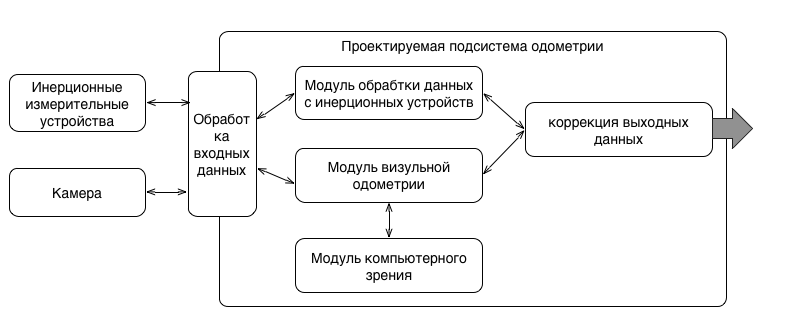
\includegraphics[width=0.8\linewidth]{pics/predmetOblast.png}}
\caption{Графическое представление процесса.}
\label{pic:predmetOblast}
\end{figure}

\paragraph{Вычисление оптического потока.}

\textbf{Оптический поток} — это изображение видимого движения объектов, поверхностей или краев сцены, получаемое в результате перемещения наблюдателя (глаз или камеры) относительно сцены\cite{wikiOpticalFlow}.

Существует несколько подходов к определению смещений между двумя соседними кадрами. Например, можно для каждого небольшого фрагмента (скажем, 8 на 8 пикселей) одного кадра найти наиболее похожий фрагмент на следующем кадре. В этом случае разность координат исходного и найденного фрагментов даст нам смещение. Основная сложность тут состоит в том, как быстро отыскать нужный фрагмент, не перебирая весь кадр пиксель за пикселем. Различные реализации этого подхода так или иначе решают проблему вычислительной сложности. Некоторые настолько успешно, что применяются, например, в распространенных стандартах сжатия видео. Платой за скорость естественно является качество. Мы же рассмотрим другой подход, который позволяет получить смещения не для фрагментов, а для каждого отдельного пикселя, и применяется тогда, когда скорость не столь критична. Именно с ним в литературе часто связывают термин “оптический поток”.

Данный подход часто называют дифференциальным, поскольку в его основе лежит вычисление частных производных по горизонтальному и вертикальному направлениям изображения. Как мы увидим далее, одних только производных недостаточно чтобы определить смещения. Именно поэтому на базе одной простой идеи появилось великое множество методов, каждый из которых использует какую-нибудь свою математическую пляску с бубном, чтобы достичь цели. Сконцентрируемся на методе Лукаса-Канаде (Lucas-Kanade), предложенном в 81 году Брюсом Лукасом и Такео Канаде. Данный метод является наименее ресурсоемким  \cite{habrOpticalFlowAbout} при этом обеспечивает приемлемое качество вычисления оптического потока. 

С математической точки зрения данный алгоритм можно описать следующим образом.
Пусть даны два изображения $F1$ и $F2$, и нам требуется найти смещение точки с координотой $x$. Рассматривая два последовательных изображения можно сказать:
$$ f_2(x) = f_1 (x-d)$$
Обратите внимание, что $f_1$ и $f_2$ при желании можно записать и в общем виде: $f_1(x) = I (x, y, t)$ ; $f_2(x) = I (x, y, t+1)$.

Свяжем известные значения со смещением d. Для этого запишем разложение в ряд Тейлора для $ f_1 (x-d)$:
$$  f_1 (x-d) =f_1(x) + df_1'(x) + O(d^2f_1'') $$
Предположим, что $ f_1 (x-d)$ достаточно хорошо аппроксимируется первой производной. Сделав это предположение, отбросим всё что после первой производной:
$$  f_1 (x-d) =f_1(x) + df_1'(x) $$

Смещение $d$ — это наша искомая величина, поэтому необходимо преобразовать $ f_1 (x-d)$ . Как мы условились ранее, $ f_2(x) = f_1 (x-d) $, поэтому просто перепишем:
$$ f_2(x)= f_1(x) - df_1'(x) $$
Отсюда следует:
$$ d = \frac{f_1(x)-f_2(x)}{f_1'(x)} $$

Следует отметить, что выше был рассмотрен одномерный случай и были сделаны несколько грубых допущений. Но описание алгоритма Лукаса-Канаде для двумерного случая только усложняет математические выводы и понимание сути. 

Для снижения погрешности вызванной отбрасыванием старших производных смещение для каждой пары кадров (назовём их $F_i$ и $F_{i+1}$) можно вычислять итеративно. В литературе это называется искажением (warping). На практике это означает, что, вычислив смещения на первой итерации, мы перемещаем каждый пиксель кадра $F_{i+1}$ в противоположную сторону так, чтобы это смещение компенсировать. На следующей итерации вместо исходного кадра $F_{i+1}$ мы будем использовать его искаженный вариант $F_{i+1}^1$. И так далее, пока на очередной итерации все полученные смещения не окажутся меньше заданного порогового значения. Итоговое смещение для каждого конкретного пикселя мы получаем как сумму его смещений на всех итерациях \cite{habrOpticalFlowTheory}.

Так же следует отметить, что данный алгоритм плохо работает на однотонных изображениях. Данный недостаток является самым критичным. 

\paragraph{Одометрия с использованием инерциальных измерительных устройств}
Навигационные решения надлежащего качества могут быть получены именно в результате взаимодействия или последующей совместной обработки данных от двух  источников - визуальной одометрии и инерциальной системы.  

В наиболее общей форме можно определить инерциальную систему как ортогональную триаду гироскопов и акселерометров, выполняющих непосредственные геопространственные измерения и вычислительный блок, осуществляющий алгоритмические преобразования данных непосредственных измерений.

Следует отметить, что гироскоп любого типа позволяет определять ориентацию в геодезическом пространстве в любой момент времени независимости от местоположения, скорости и других параметров носителя. Точность поставляемых гироскопом данных во всех случаях подвержена деградации («ухода») с течением времени. Величина «ухода» значительна и может составлять до нескольких градусов в час \cite{laserLocation}.

Акселерометры предназначены для измерения линейных ускорений. В равной степени они пригодны для измерений сил, так как согласно ньютоновской механике сила и ускорение есть разные проявления одного и того же физического явления.

В общем случае в системах навигации следует определять следующие показатели:
\begin{itemize}
\item \textbf{Рыскание} — угловые движения летательного аппарата, судна, автомобиля относительно вертикальной оси (см. также вертикальная ось самолёта), а также небольшие изменения курса вправо или влево, свойственные судну \cite{wikiRiskanie};
\item \textbf{Крен} — поворот объекта (судна, самолёта, фундамента) вокруг его продольной оси \cite{wikiKren};
\item \textbf{Тангаж} — угловое движение летательного аппарата или судна относительно главной (горизонтальной) поперечной оси инерции \cite{wikiTangazh}.

\end{itemize}
С учетом сделанных замечаний рассмотрим основные процедуры, выполняемые в навигационном комплексе на базисном уровне.

\textit{\textbf{Вычисление крена и тангажа посредством акселерометров}}

Обладая чувствительностью к земной гравитации, акселерометры обеспечивают измерение долговременных значений крена и тангажа по схеме, изображенной на рисунке~\ref{pic:tangazh}. Рассмотрим акселерометр, рабочая ось которого совпадает со строительной осью $oX$ носителя.

\begin{figure}[!htb]
\center{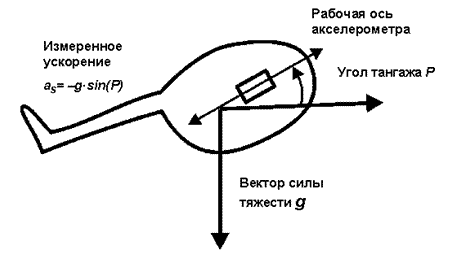
\includegraphics[width=0.6\linewidth]{pics/tangazh.png}}
\caption{Измерения величин крена и тангажа посредством акселерометров.}
\label{pic:tangazh}
\end{figure}

Полагая ускорение носителя равным нулю, мы можем вычислить угол тангажа как:
$$P = \arcsin (-a_s/g)$$

Аналогично вычисляется угол крена. Таким образом, два из трех углов, определяющих угловую ориентацию, могут быть определены только за счет использования акселерометров. Это совершенно очевидный результат, принимая во внимание то обстоятельство, что углы крена и тангажа по изначально определены по отношению к вертикали, которая в нашем случае соответствует вектору тяжести. Однако, здесь следует признать, что описанный метод не может быть использован на практике сам по себе, так как в описанной схеме существенно состояние покоя, в котором должна находиться система. Если это условие не соблюдается, то совершенно очевидно, что отсутствует принципиальная возможность выделить вектор ускорения свободного падения из суммы всех ускорений, которую испытывает система.

\textit{\textbf{Вычисление изменений ориентации с использованием гироскопов}}

Как отмечено выше, в конструкции навигационного комплекса используются оптические гироскопы, обладающие чувствительностью к изменениям ориентации т.е. к величине угловой скорости. Интегрирование (численное суммирование) значений, измеренных гироскопами, обеспечивает определение кратковременных угловых перемещений в физическом пространстве.

Для корректного расчета угла поворота должны быть учтены
внутренние ошибки гироскопа – дрейф, ошибка масштабного коэффициента, случайный шум.

При этом внутренние ошибки  гироскопа полностью смешаны с истинными значениями и не могут быть отделены от них на базисном информационном уровне. В процессе дальнейшей обработки эта смесь подвергается интегрированию, в результате чего возникает ошибочное угловое смещение, которое, таким образом, приобретает долговременный характер (рис. ~\ref{pic:acell}). Точная оценка величины ошибочного углового смещения и его устранение осуществляется при генерации навигационного решения на последующем навигационном уровне.

\begin{figure}[!htb]
\center{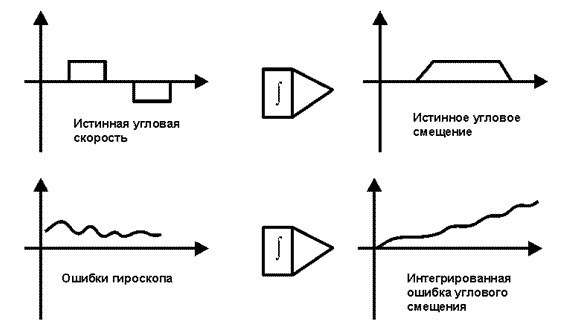
\includegraphics[width=0.6\linewidth]{pics/acelerometr.png}}
\caption{Схема определения углового смещения.}
\label{pic:acell}
\end{figure}

\textit{\textbf{Определение координат пространственного положения с помощью акселерометров.}}

Наличие акселерометров позволяет определять величины линейных ускорений, которые испытывает система. Положим, что ориентация системы в физическом пространстве определена точно с помощью методов, описанных выше. Тогда имеется возможность выделить вектор силы гравитации среди всей суммы векторов сил, приложенных к системе и, следовательно, оценить величину ускорения. Численное интегрирование ускорения позволяет перейти к скорости, а повторное интегрирование к перемещению. Таким образом, с учетом представленных выше замечаний и правилах перехода из физического пространства в географическое, появляется принципиальная возможность оценить геодезические координаты системы в любой момент времени.

\paragraph{Корректировка выходных данных}

\paragraph{Анализ функций, подлежащих автоматизации}

\subsubsection{Выбор критериев качества}
Выделим основные критерии, по которым следует оценивать разрабатываемую подсистему.
\begin{itemize}
\item \textbf{Необходимость в специальном оборудовании} - исходя из задачи, предполагается использование проектируемого модуля в низкобюджетных системах. В связи с этим необходимо обеспечить корректную работу подсистемы с неспециальным оборудованием таким, как бытовые камеры. 
\item \textbf{Стоимость необходимого оборудования} – исходя из предыдущего пункта, следует обеспечивать поддержку наиболее дешевого оборудования. 
\item \textbf{Сложность интеграции} – в современном мире наличия многих конкурентов и налогов одним из ключевых факторов при выборе между ними является простота использования продукта. В связи с этим необходимо снизить время, необходимое на интеграцию с разрабатываемой подсистемой, путем предоставления удобного в использовании API.
\item \textbf{Точность} - данный критерия является важным для задач определения положения в пространстве априори, так как при низкой точности использование систем данного рода становится бесмысленным. Тем не менее в рамках многих задач обеспечение чрезмерно высокой точности является избыточным.
\item \textbf{Возможность свободного использования} – нередко разработчики программных или аппаратных продуктов накладыают ограничение в виде разного рода лицензий распространения, которые ограничивают пользователей в распространении и использовании своих продуктов. В связи с этим важным явлется свободность использования продукта в любых целях, не  противоречящих законодательству стран, где проихсходит его использование.
\end{itemize}

\subsubsection{Анализ аналогов и прототипов}


\paragraph{Сравнительный анализ}

Для сравнения представленных вариантов воспользуемся методом взвешенной суммы. Данный метод позволяет объединить ряд критериев сравнения в один интегральный показатель, по которому затем выбирается наилучший вариант, соответствующий максимальному значению этого интегрального показателя. Метод взвешенной суммы можно представить следующим образом: 
$$ Y = \max_{j \ni m} \displaystyle\sum_{i=1}^{n} \alpha_i \cdot K_{ij},$$
где $\sum_{i=1}^{n} \alpha_i = 1$

По этому критерию проводится сравнение $j (j = 1, 2, …, m)$ вариантов по $i (i = 1, 2, …, n)$ показателям, где:

$n$ – количество показателей сравнения;

$m$ – количество вариантов сравнения.

$K_{ij}$ – нормированный коэффициент соответствия $i$-ого параметра $j$-ого варианта эталонному значению, т.е. для $j$-ого варианта:
$$ K_{ij} = \frac{\max_{j} X_{ij}} {X_{ij}}, $$
$$ 0 < K_{ij} < 1 $$
Соответствие систем-аналогов выбранным критериям качества представлено в Таблице

\subsubsection{Перечень задач, подлежащих решению в процессе разработки}

Исходя из приведенного выше первичного анализа предметной области можно сформировать список задач, подлежащих решению.

Необходимо решить следующие задачи:

\begin{enumerate}
\item разработка структуры и архитектуры подсистемы системы; 
\item разработка требований к формату и структуре передаваемых данных;
\item разработка алгоритмов обработки информации;
\item выбор и обоснование КТС, необходимого для реализации системы;
\item разработка графа диалога и набора экранных форм;
\item оценка предполагаемого качества функционирования системы;
\item организационно-экономическое обоснование разработки;
\item рекомендации по охране труда.
\end{enumerate}





\subsection{Проектирование подсистемы}
\subsubsection{Разработка структуры подсистемы}
\paragraph{Определение состава компонентов}

Исходя из анализа функций структурно в подсистеме можно выделить следующие основные части:
\begin{itemize}
\item \textbf{модуль обработки входных данных} (преобразует входные данные в удобоваримый вариант для последующей обработки);
\item \textbf{модуль компьютерного зрения }(позволяет обрабатывать изображения и производить их анализ для построения визуальной одометрии);
\item \textbf{модуль визуальной одометрии} (высчитывает перемещение и угол поворота камеры на основе последовательности изображений);
\item \textbf{модуль обработки данных с инерционных приборов} (производит математическую обработку показаний датчиков и на ее основе вычисляет перемещение объекта);
\item \textbf{модуль сопоставления  и вывода данных} (сравнивает показания двух предыдущих модулей и на их основе выводит наиболее правдоподобное положение объекта).
\end{itemize}

\paragraph{Определение структуры компонентов}
Согласно общепринятой терминалогии система состоит из подсистем, а те в свою очередь из модулей. Таким образом разрабатываемая подсистема состоит из следующих модулей:

\begin{itemize}
\item обработки входных данных;
\item обработки выходных данных;
\item визульной одометрии;
\item компьютерного зрения;
\item настроек;
\item одометрии на основе инерционных устройств.
\end{itemize}

Графически архитектура подсистемы представлена на рисунке~\ref{pic:acrhitec}.

\begin{figure}[!htb]
\center{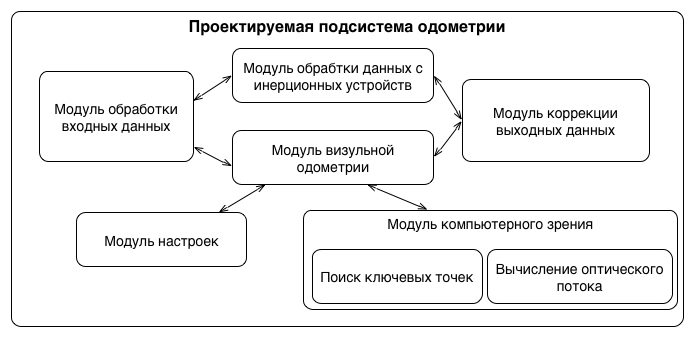
\includegraphics[width=0.8\linewidth]{pics/achitecture.png}}
\caption{Структура компонентов.}
\label{pic:acrhitec}
\end{figure}

\textbf{Назначение модулей}

\begin{itemize}
\item \textbf{Модуль обработки входных данных} - нормализует входные данные и аккумулирует их, в случае слишком высокой частоты их поступления.
\item \textbf{Модуль обработки выходных данных} - сравниевает данные, полученные независимо в модуле визуальной одометрии и в модуле обработки данных с ИИУ, и принимает решение об их корректности на основе определенных сигнальных показателей (см. пункт~\ref{item:outputCorrect}).
\item \textbf{Модуль визуальной одометрии} – вычисляет перемещения на основе видеоряда. Для обработки видео использует модуль компьютерного зрения. 
\item \textbf{Модуль компьютерного зрения} – реализует стандартные алгоритмы компютеного зрения, такие как вычисление оптического потока, поиск опорных точек на изображении, трансформация и измениние изображений.
\item \textbf{Модуль одометрии на основе инерционных устроств} – производит расчеты перемещения обхекта на основе полученных данныз с гироскопов и акселерометров.
\item \textbf{Модуль настроек} - содержит в себе данные об используемом оборудовании и его характеристиках. Эти данные используются в модулях одометрии. 
\end{itemize}

\paragraph{Описание процессов}
В ходе работы всей подсистемы протекает множество процессов по обработке и преобразованию информации. Выделим ключевые из них.

\textbf{Визуальная одометрия.}

В данной работе делается упор на создание визуальной одометрии на основе одной бытовой камеры и относительно слабых вычислительных устройств. Такое решение требует соблюдения двух условий, которые приемлемы при создании большинства современных мобильных роботов:
\begin{enumerate}
\item перемещение происходит по земле или другой горизонтальной плоскости;
\item камера жестко закреплена относительно самого носителя.
\end{enumerate}

При соблюдении этих условий работу визуальной одометрии можно описать в 8 шагов\cite{visaulOdometryMy}.
\begin{enumerate}
\item Исправление изображения для исключения искажения линз.
\item Вычисление оптического потока для кадра.
\item Проверка полученных векторов смещения, исключение движущихся в кадре объектов, исключение ошибочных векторов.
\item Разделение всего оптического потока на две части: «наземную» и «небесную».
\item В «небесной» части перейти к цилиндрической системе координат и высчитать угол поворота относительно двух последних кадров, определяя тем самым угол поворота $\theta$.
\item В «наземной» части выделить векторы $(u,v)$ из оптического потока  и вычислить перемещение в плоскости x-y , получив вектор $(x, y)$.
\item Прибавить $(x, y, \theta)$ к изначальному положению объекта $(X, Y, \Theta)$, получив новое положение объекта.
\item Перейти к шагу 1 для следующего кадра. Периодически обновлять ключевые точки.
\end{enumerate}
	
В общем виде процесс вычисления оптического потока представлен на рисунке~\ref{pic:visOdometryProc}.

\begin{figure}[!htb]
\center{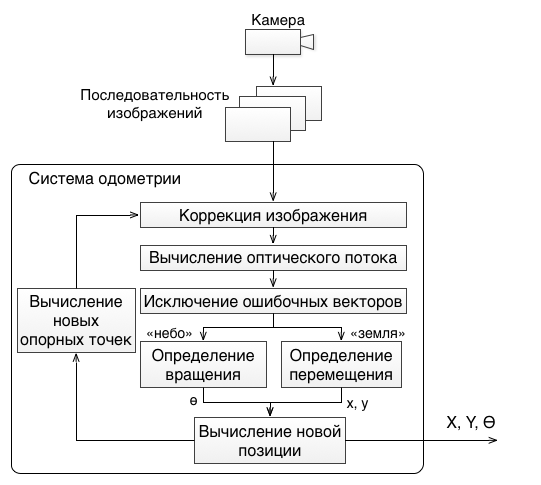
\includegraphics[width=0.8\linewidth]{pics/visualOdometryProcess.png}}
\caption{Графическое представление процесса визуальной одометрии}
\label{pic:visOdometryProc}
\end{figure}

\textbf{Обработка данных с инерционных измерительных устроств.}

Обработка данных с инерционных устройств представляет собой несколько операций интегрирования полученных данных. 
Рассмотрим переход от ускорений к перемещению.

Пусть на выходе акселерометра снимаются ускорения $Z_a$, $Y_a$ и $Z_a$, которые показывают ускрения по осям $X$, $Y$, $Z$.

Как мы знаем из курса физики, $ \int_a^b a(t)dt = V(t)+C $.
В то же время $ \int_a^b V(t)dt = S(t)+C $. Таким образом получаем:
$$
\iint_a^b a(t)dt = \int_a^b V(t) + C_v = S(t) + C_v \cdot t + C_s 
$$.

Так как $С_s$ в нашем случае, это начальное положение носителя, то его мы принимаем = 0. Отсюда получаем формулу:
$$
\iint_a^b a(t)dt = \int_a^b V(t) + C_v = S(t) + C_v \cdot t .
$$

Однако все упрощается, если период замеров настолько мал, что ускорение можно считать равномерным. Тогда формулы преобретают следующий вид:
$$ V_t = V_{t-1} + a_t \cdot t$$
$$ S_t = S_{t-1} + V_t \cdot t $$

Графически это можно выразить тремя графиками (рис.~\ref{pic:integral}): показывающими рассчитанное значения пермещения и сокрости в зависимости от времени. 

\begin{figure}[!htb]
\center{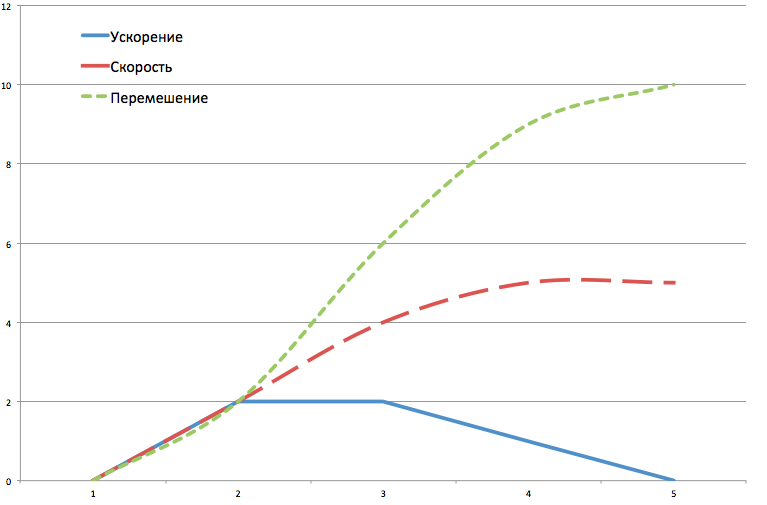
\includegraphics[width=0.8\linewidth]{pics/integrals.png}}
\caption{Пример интегрирования ускорения для получения перемещения}
\label{pic:integral}
\end{figure}


Производя подобные математические вычисления для координат $X$ и 
$Y$ получаем перемещения по этим координатам. Причем мы можем опускать финальную константу интегрирования, так как нам необходимо определить не пройденный путь от начала движения, а именно путь, пройденный за последнний временной отрезок. 

Аналогично обрабатываются данные с акселерометров, с одинм лишь отличием - акселерометры могут предоставлять сразу угловую скорость, что позволяет производить лишь одно интегрирование.


\paragraph{Математическое обеспечение}\label{math}

В рамках данной работы многие процессы основываются на фундаментальных исследованиях в области компьютерного зрения и обработки изображений. Далее рассматриваются основные из них.

\textbf{Поиск ключевых точек}

Есть много видов местных ключевых точек, которые можно отслеживать. Для начала стоит рассмотреть что из себя представляет ключевая точка сама по себе (ключевая особенность изображения). Очевидно, что если мы выбираем точку на большой однотонной стене, то будет не легко найти, что же точку в следующем кадре из видео.

Если все точки на стене могут быть одинаковыми или даже очень похожи, то у нас будет мало шансов отслеживания этой точки в последующих кадрах. С другой стороны, если мы выберем точку, которая является уникальной, то у нас будут довольно хорошие шансы снова найти эту точку. На практике, точка или черта, которая мы выбираем в качестве клюевой должны быть уникальным или почти уникальны, и должна быть параметризуемой таким образом, чтобы ее можно было отличить от других точек на изображении.

Возвращаясь к нашей аналогии с большой пустой стеной, мы могли бы попытаться искать точки, которые имеют некоторые значительные изменения в окрестности, например, большую производную. На практике оказывается, что этого не достаточно. Точка, в которой большое значение производной, может находиться на какой-то линии, но все точки на этой линии будут иметь такую же или близкую производную.

Однако, если высокие значения производные наблюдаются в двух ортогональных направлениях, то можно надеяться, что эта точка будет уникальной. По этой причине, такие особенности на изображении называются углами. Очевидно, углы - не края - это точки, которые содержат достаточно информации, чтобы ее нашли на последующих кадрах.

Определение углов опирается на матрице производных второго порядка 
$(\partial^2 x, \partial^2 y, \partial x \partial y)$ интенсивностей изображения. Эта терминология происходит от матрицы Гессе вокруг точки, которая определяется в двух измерениях следующим образом:

$$ 
H(p) = 
\begin{bmatrix} 
	\frac{\partial^2 I}{\partial x^2} & \frac{\partial^2 I}{\partial x \partial y}  \\ 
 	 \frac{\partial^2 I}{\partial x \partial y} & \frac{\partial^2 I}{\partial y^2} 
\end{bmatrix}
$$

Такие углы, по определению Харриса, места на изображении, где автокорреляционная матрица вторых производных имеет два больших собственных значения. По сути, это означает, что есть текстуры или грани , идущие, по крайней мере, в двух отдельных направлениях, сосредоточенные вокруг такой точки, так же, как реальные углы имеют по крайней мере два ребра, сходящихся в точку. Использование вторых производных позволяет точно определить особенности, потому что они не отвечают единым градиентами(так как при первой производной равной константе, вторая будет равна нулю). Это определение имеет дополнительное преимущество, в том, что когда мы рассматриваем только собственных значений автокорреляционной матрицы, мы рассматриваем величины, инвариантные также к вращению, что является важным, потому что объекты, которые мы отслеживаем могут вращаться, а также перемещаться. Следует также отметить, что эти два собственных значения делают больше, чем просто определяют, является ли точка перспективной для обслеживания - они также обеспечивают идентифицирующую роль для точки.

В используемом в данной работе пакете компьютерного зрения используется функция  $cvGoodFeaturesToTrack()$.
\begin{verbatim}
void cvGoodFeaturesToTrack(
        const CvArr* image,
        CvArr* eigImage, CvArr* tempImage,
        CvPoint2D32f* corners,
        int* cornerCount,
        double qualityLevel,
        double minDistance,
        const CvArr* mask=NULL,
        int blockSize=3,
        int useHarris=0,
        double k=0.04 
);
\end{verbatim}
Эта функция вычисляет воторые производные для точек и их собственные значения. Результатом работы функции является список точек, которые являются хорошими кандидатами для ключевых точек.

\textbf{Оптический поток}

Задача вычисления оптического потока можно сформулировать следующим образом: оценить движение между двумя кадрами не имея никакой информации о происходящем, кроме самих кадров\cite{OpenCVBook}. 

Вычисля оптический поток, мы можем связать для каждого пикселя определить некий ветктор смешения, которые будут показывать куда переместился пиксель между предыдущим кадром и текущим кадром. Такой  подход обычно называют плотным оптическим потоком, который определяет перемещение каждого пикселя. Метод Хорн-Шунка (Horn-Schunck) вычисляет именно такой оптический поток. В его основе лежит один, казалось бы, простой принцип - просто пытаться найти наиболее похожий пиксель на следующем кадре в пределах какого-то окна вокруг исходного пикселя.

На практике расчет плотного оптического потока затруднителен. Рассмотрим движение белого листа бумаги. Многие из белых пикселей в предыдущем кадре просто остаются белыми на следующих. Изменения будут лишь на границах листа, и то, только вокруг гарниц перпендикулярных движению. В результате необходимо прибегать к различным математическим приемам, что сказывается на увеличении ресурсоемкости операции в целом. 

Это приводит нас к альтернативному варианту, выборочный оптического потока. Алгоритмы такого рода опираются на некоторые средства определения заранее подмножество точек, которые должны быть отслежены. Если эти точки имеют определенные свойства, такие как свойства ключевых особенностей, обсуждаемые ранее, тогда отслеживая будет относительно точным и надежными. Для многих практических случаев, вычислительная стоимость выборочного оптичкского потока намного меньше, чем у плотного оптического потока, поэтому последнему отводится только академический интерес.

Рассмотрим наиболее популярный метод вычисления выборочного оптического потока - метод Лукаса-Канаде (Lucas-Kanade). Этот метод также имеет реализацию, которая работает с пирамидами изображений, что позволяет нам отслеживать быстрые движения. В данной работе используется именно он, так как он обладает наиболее низкой вычислительной сложностью. 

{\large \textit{\textbf{Метод Лукаса-Канаде}}}

Метод (алгоритм) Лукаса - Канаде (ЛК) создавался в 1981 году и первоначально задумывался для вычисления плотного оптического потока. Тем не менее, Алгоритм работал и с любым количеством точек для отлеживания, что позволило использовать его в столь важных выборочных оптических потоках. 

Алгоритм ЛК может быть применен для определнного числа точек, потому что он опирается только на локальной информации о точке, которая является производной в некотором маленьком окне вокруг каждой из ключевых точек. Недостатком использования небольших локальных окон в ЛК является то, что большие смещения могут перемещать точки за пределы таких локального окон, что приведет к невозможности их нахождения. Эта проблема привела к разработке "пирамидальной" версии алгоритма, которая составляет пирамиду из нескольких копий изображения разного размера, после чего вычисляет оптический поток, начиная с самого высокого уровня в пирамиде изображений, постепенно опускаясь по уровням для более высокой точности. 

\begin{figure}[!htb]
\center{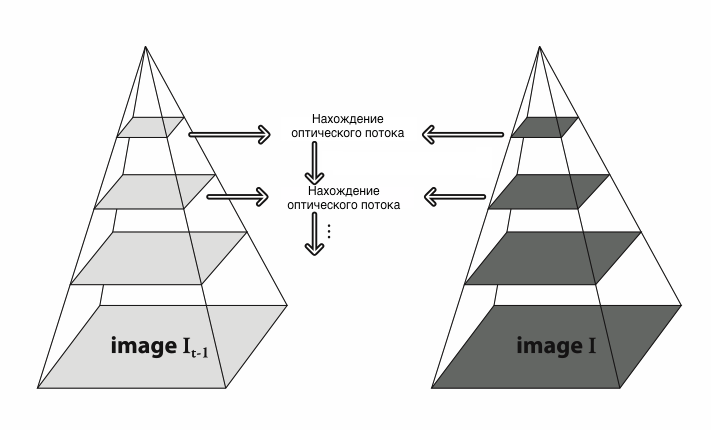
\includegraphics[width=0.8\linewidth]{pics/pyrLK.png}}
\caption{Графическое представление работы "пирамидальной" версии алгоритма ЛК}
\label{pic:pyrLK}
\end{figure}

\textbf{Принцип работы алгоритма}

Основная идея алгоритма ЛК основывается на трех предположениях. 
\begin{enumerate}
\item \textit{Яркость постояна.} Предполагается, что пиксель не меняет внешний вид, переходя от кадра к кадру. Для изображений в градациях серого (для случая с цветными изображениями есть более строгое допущение, но оно сводится к этому) это означает, что яркость пикселя не меняется, при его отслеживании от кадра к кадру. 
\item \textit{Малые сдвиги}. Изображение двигается медленно во времени. На практике это означает, что объект от кадра к кадру сдвигается незанчительно.
\item \textit{Пространственная когерентность.} Соседние точки в кадре принадлежат к одной и той же поверхности и имеют аналогичные смещения.
\end{enumerate}

Из первого допущения следует:
$$
f(x, t) \equiv I(x(t), t) = I(x(t+dt), t + dt)
$$

Отсюда следует, что интенсивность отслеживаиваемых пикселей не измененяется с течением времени:
$$
\frac{\partial f(x)}{\partial t} = 0
$$

Второе предположение, по существу, означает, что движения от кадра к кадру крайне малы. Другими словами, мы можем рассматривать это изменение как аппроксимацию производной от интенсивности по времени. Чтобы понять последствия этого предположения, рассмотрим сначала случай одного пространственного измерения.
Запишем уравнение яркости $F(x,t)$ с учетом зависимости $x$ от $t$ и применим правило частного дифференцирования:
$$
\underbrace{\frac{\partial I }{\partial x} \Bigr|_t}_{I_x} 
\underbrace{\left( \frac{\partial x }{\partial t} \right)}_{V} + 
\underbrace{\frac{\partial I }{\partial t} \Bigr|_{x(t)}}_{I_t} =
 0,
$$

где $I_x$ является пространственной производной по первому изображению, $I_t$ это производная между изображениями в течение долгого времени, и $V$ -скорость, которую мы ищем. Таким образом, мы приходим к простому уравнению для скорости оптического потока в простой одномерной случае:

$$ V = \frac{I_t}{I_x} $$

Рассмотрим стандартную задачу в одномерном случае. На рисунке~\ref{pic:OptFlow1D} представлена ее графическая иллюстрация. Кривая $I(x, t)$ изображает некую грань, слева от которой значения интенсивности высоки, а справа - низкие. Необходимо определить как сдвинулась это грань на следующем кадре. 

\begin{figure}[!htb]
\center{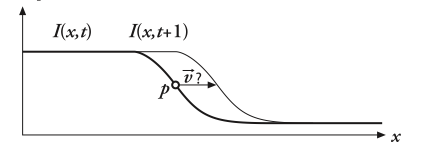
\includegraphics[width=0.8\linewidth]{pics/optFlow1D.png}}
\caption{Графическое представление задачи нахождения оптического потока в одномерном случае.}
\label{pic:OptFlow1D}
\end{figure}

На рисунке~\ref{pic:OptFlow1DSolve} показано как можно решить такую задачу. При учете двух первых предположений  получим следующее:
$$
I_x = \frac{\partial I}{\partial x} \Bigr|_t \; и \;
I_t = \frac{\partial I}{\partial t} \Bigr|_{x=p} \Rightarrow 
\vec{V} \approx - \frac{I_t}{I_x}
$$
\begin{figure}[!htb]
\center{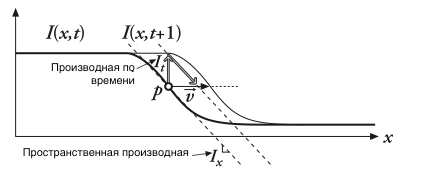
\includegraphics[width=0.8\linewidth]{pics/OptFlow1DSolve.png}}
\caption{Графическое представление решения задачи нахождения оптического потока в одномерном случае.}
\label{pic:OptFlow1DSolve}
\end{figure}

Теперь рассмотрим двумерный случай. Будем обозначть $u_y$ скорость вдоль оси $Y$, а $u_x$ -вдоль $X$:
$$ I_xu +I_yv+I_t = 0 \equiv 
\frac{\partial I}{\partial t} + 
u_x \cdot \frac{\partial I}{\partial x} + 
u_y \cdot \frac{\partial I}{\partial y} = 0 
$$

Полученное уравнение, говорит нам о том, что сумма частных производных должны быть равна нулю. Но вознакает проблема - уравнение у нас одно, а неизвестных в нем два: $u_x$ и $u_y$.

Воспользовавшись третьим предположением, о том, что соседние пиксели смещаются на одинаковое расстояние, запишем это же уравнение для окна 5х5 пикселей, получив 25 уравнений. Очевидно, что 3 допущение не всегда верно, поэтому в общем случае система не имеет решения поэтому перейдем к минимизации ошибки:

$$
E(u_x, u_y) = \sum \limits_{i,j} g(x_i, y_i) 
\left[ \frac{\partial I}{\partial t} + 
u_x \cdot \frac{\partial I}{\partial x} + 
u_y \cdot \frac{\partial I}{\partial y} \right]^2
$$

Здесь $g$ — это функция, определяющая весовые коэффициенты для пикселей. Самые распространенный вариант — двумерная гауссиана, которая дает наибольший вес центральному пикселю и все меньший по мере удаления от центра (см. рис.~\ref{pic:Gaussian2d}).

\begin{figure}[!htb]
\center{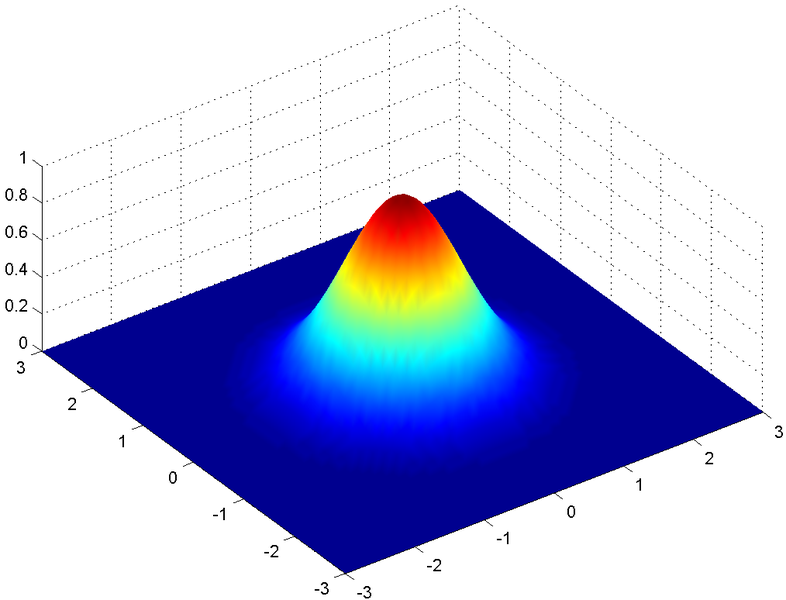
\includegraphics[width=0.8\linewidth]{pics/Gaussian2d.png}}
\caption{Двумерная гауссиана}
\label{pic:Gaussian2d}
\end{figure}

Чтобы найти минимум  $E(u_x, u_y)$ воспользуемся методом наименьших квадратов, найдем её частные производные по $u_x$ и $u_y$ и запишем в более компактной форме, приравням к 0:

$$
\frac{\partial E(u_x, u_y) }{\partial u_x} = 
\sum \limits_{i,j} g(x_i, y_i) 
\left[
u_x \left( \frac{\partial I}{\partial x} \right)^2 +
	u_y \frac{\partial I}{\partial y}\frac{\partial I}{\partial x} +
	\frac{\partial I}{\partial x}\frac{\partial I}{\partial t}
\right] = 0
$$

$$
\frac{\partial E(u_x, u_y) }{\partial u_y} = 
\sum \limits_{i,j} g(x_i, y_i) 
\left[
	u_x \frac{\partial I}{\partial y}\frac{\partial I}{\partial x} +
	u_y \left( \frac{\partial I}{\partial y} \right)^2 +
	\frac{\partial I}{\partial x}\frac{\partial I}{\partial t}
\right] = 0
$$

Перепишем эти два уравнения в матричной форме:
$$ M \vec{u} = \vec{b}$$

Где: 
$$ M = 
\left[ 	
\begin{array}{cc}
	\sum \limits_{i,j} g(x_i, y_i) 
		\left( \frac{\partial I}{\partial x} \right)^2 
	& \sum \limits_{i,j} g(x_i, y_i) 
			\frac{\partial I}{\partial x} 										\frac{\partial I}{\partial y} 
	\\ 
	\sum \limits_{i,j} g(x_i, y_i) 
			\frac{\partial I}{\partial x} 										\frac{\partial I}{\partial y} 
	& \sum \limits_{i,j} g(x_i, y_i)
		\left( \frac{\partial I}{\partial y} \right)^2 
\end{array} 
\right]
$$

$$
\vec{b} = -
\left[ 	
\begin{array}{c}
\sum \limits_{i,j} g(x_i, y_i) 
			\frac{\partial I}{\partial t} 										\frac{\partial I}{\partial x}  \\ 
\sum \limits_{i,j} g(x_i, y_i) 
			\frac{\partial I}{\partial t} 										\frac{\partial I}{\partial y}
\end{array} 
\right]
$$

$$
\vec{u} = 
\left[ 	
\begin{array}{c}
  u_x\\ 
	u_y
\end{array} 
\right]
$$

Если матрица М обратима (имеет ранг 2), можем вычислить $u_x$ и $u_y$ , которые минимизируют ошибку $E$\cite{habrOpticalFlowAbout}:
$$
\widehat{u} = M^{-1} \cdot \vec{b}
$$

\textbf{Калибровка камеры}
Еще одиним математическим аспектом данной работы является калибровка камеры. 

\textit{\textbf{Калибровка камеры}} — это задача получения внутренних и внешних параметров камеры по имеющимся фотографиям или видео, отснятым ей\cite{wikiCalibrate}.

Рассмотрим простейшую модель камеры, модель камеры с тонкой линзой. В этой простой модели, свет рассматривается в качестве потка от сцены или удаленного объекта, но только один луч попадает из любой конкретный точки этого объекта. Все эти точки проецируются на матрицу камеры или другую поверхность изображения. В результате, изображение на этой плоскости изображения всегда в фокусе, а масштаб изображения относительной его раельного размера определяется одним параметром камеры -  его фокусным расстоянием. На рисунке~\ref{pic:cameraModel} схематично показана рассматриваемая модель камеры\cite{openCVBook}. 

\begin{figure}[!htb]
\center{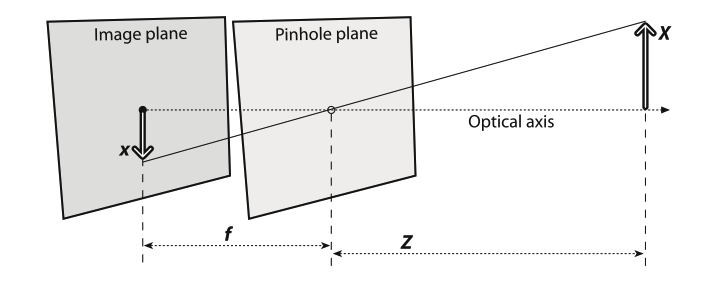
\includegraphics[width=0.8\linewidth]{pics/cameraModel.png}}
\caption{Модель камеры с тонкой линзой}
\label{pic:cameraModel}
\end{figure}

Из изображения видно, что, на основе подобия треугольников, $-x/f = X/Z$:
$$	-x = f \cdot \frac{X}{Z} $$

Учитывая тот факт, что главная оптическая ось пересекает плоскость изображения не в координате $(0,0)$, в координате $с$ получим:

\begin{equation}
\label{formula:focus}
-x = f \cdot \frac{X}{Z} + с
\end{equation}

Далее будем рассматривать именно цифровые камеры с ПЗС-матрицами. У данных камер есть одна особенность - пиксели матрицы не квадратной формы из-за технологических условий изготовления. Учитывая этот факт, распишем уравнение (\ref{formula:focus}) для координат $x$ и $y$:

$$ u = f \cdot s_u \cdot \frac{X}{Z} + c_u $$
$$ v = f \cdot s_v \cdot \frac{X}{Z} + c_v $$

где $s_u$ и $s_v$ - коэффициенты формы пикселя.



\subsubsection{Разработка формата и структуры данных}
В ходе функционирования подсистемы информация поступает на ее вход, получается на ее выходе, и передается между модулями внутри системы. 
При этом эта информация носит разные характер и смысл. Так как подсистема носит сугубо программный характер, то все потоки даных реализуются только программными средствами, в виде структур данных. Сетевые технологии не накладывают никаких ограничений на форматы информационных структур. 
Ниже дано описание основных форматов обмена информацией.

\begin{itemize}
\item \textbf{Видео (вход)}. Видео подается на вход системы покадрово, в связи с этим алгоритм кодирования и сжатия видео не существеннен, так как задача сформировать следующий кадр в его полном объеме ложиться на вызывающую стороную. По сути, каждый кадр представляет собой 1 картинку в формате JPEG, что проще всего представать матрицей, размер которой соответствует размеру кадра, а ее элементами являются структуры данных, хранящие информацию о каналах изображения. 

\item \textbf{Ускорения по трем осям (вход)}. Данные подаваемые с акселерометров или одного, трехосевого акселерометра. Данные имеют цифровое представления, дробное. 

\item \textbf{Угловое ускорение по трем осям (вход)}. Данные подаваемые с гироскопов или одного, трехосевого гиросокопа. Данные имеют цифровое представления, дробное. 

\item \textbf{Текущие координаты и угол поворота (выход)}. Высчитанное на текущей итерации положение объекта. Две координаты $X$ и $Y$ представляют собой целые числа. Угол поворота  $\alpha$- дробное число. Аналогиным образом можно представлять информацию о смещениях, полученных на текущей итерации. 

\item \textbf{Информационный обмен между модулем визуальной одометрии и модулем компьютерного зрения}. Данный информационых обмен происходит два раза за итерацию: для нахождения ключевых точек на кадре и для вычисления оптического потока. При этом в разных случаях содержание информационных сообщений будет разное.
	\begin{itemize}
	\item Нахождение ключевых точек - от модуля визуальной одометрии поступает изображение, являющееся кадром. Пресдставляет собой матрицу, размер которой соответствует размеру кадра, а ее элементами являются структуры данных, хранящие информацию о каналах изображения. В ответ модуль компьютерного зрения возвращает список точек в формате ${x, y}$, где $x$ и $y$ - позиция пикселя на изображении при начале отсчета в левом верхнем углу. 
	
	\item Вычисление оптического потока - от модуля визуальной одометрии поступает два изображения (текущий и предыдущий кадры)и список ключевых точек. Представление соответствует описаному ранее. В ответ модуль компьютерного зрения возвращает два списка: список смещений, представляющий собой список пар $\triangle x, \triangle y$, и вектор ошибок, состоящий из 0 и 1 - 1 означает, что соотвествующая ключевая точка не была найдена на втором изображении и вектор смещения найден ошибочно или не найден вообще. 
	
	\end{itemize}
\end{itemize}

\subsubsection{Разработка алгоритмов обработки информации}
\paragraph{Общий алгоритм работы}
\paragraph{Алгоритм вычисления оптического потока}
\paragraph{Алгоритм обработки данных с ИИУ}
\paragraph{Алгоритм сопоставления и корректировки выходных данных}

